% Created by tikzDevice version 0.12.6 on 2024-11-19 16:55:30
% !TEX encoding = UTF-8 Unicode
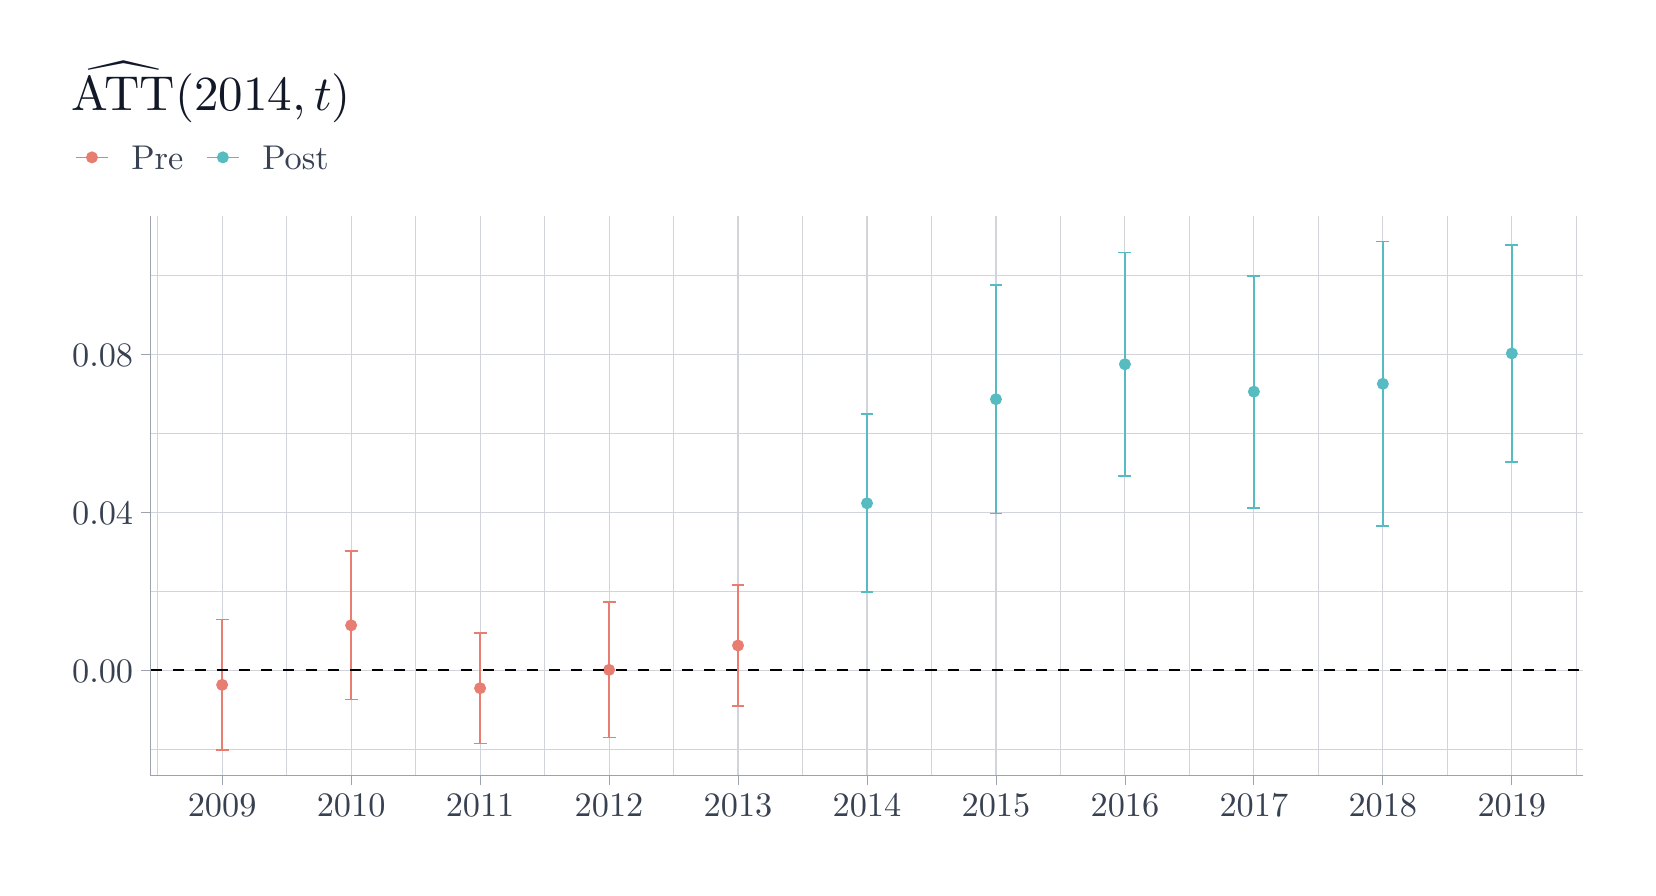
\begin{tikzpicture}[x=1pt,y=1pt]
\definecolor{fillColor}{RGB}{255,255,255}
\path[use as bounding box,fill=fillColor] (0,0) rectangle (578.16,303.53);
\begin{scope}
\path[clip] (  0.00,  0.00) rectangle (578.16,303.53);
\definecolor{drawColor}{RGB}{255,255,255}

\path[draw=drawColor,line width= 0.7pt,line join=round,line cap=round,fill=fillColor] (  0.00,  0.00) rectangle (578.16,303.53);
\end{scope}
\begin{scope}
\path[clip] ( 44.41, 33.29) rectangle (562.16,235.43);
\definecolor{drawColor}{RGB}{255,255,255}
\definecolor{fillColor}{RGB}{255,255,255}

\path[draw=drawColor,line width= 0.7pt,line join=round,line cap=round,fill=fillColor] ( 44.41, 33.29) rectangle (562.16,235.43);
\definecolor{drawColor}{RGB}{209,213,219}

\path[draw=drawColor,line width= 0.4pt,line join=round] ( 44.41, 42.79) --
	(562.16, 42.79);

\path[draw=drawColor,line width= 0.4pt,line join=round] ( 44.41, 99.82) --
	(562.16, 99.82);

\path[draw=drawColor,line width= 0.4pt,line join=round] ( 44.41,156.85) --
	(562.16,156.85);

\path[draw=drawColor,line width= 0.4pt,line join=round] ( 44.41,213.88) --
	(562.16,213.88);

\path[draw=drawColor,line width= 0.4pt,line join=round] ( 46.97, 33.29) --
	( 46.97,235.43);

\path[draw=drawColor,line width= 0.4pt,line join=round] ( 93.58, 33.29) --
	( 93.58,235.43);

\path[draw=drawColor,line width= 0.4pt,line join=round] (140.18, 33.29) --
	(140.18,235.43);

\path[draw=drawColor,line width= 0.4pt,line join=round] (186.78, 33.29) --
	(186.78,235.43);

\path[draw=drawColor,line width= 0.4pt,line join=round] (233.38, 33.29) --
	(233.38,235.43);

\path[draw=drawColor,line width= 0.4pt,line join=round] (279.98, 33.29) --
	(279.98,235.43);

\path[draw=drawColor,line width= 0.4pt,line join=round] (326.59, 33.29) --
	(326.59,235.43);

\path[draw=drawColor,line width= 0.4pt,line join=round] (373.19, 33.29) --
	(373.19,235.43);

\path[draw=drawColor,line width= 0.4pt,line join=round] (419.79, 33.29) --
	(419.79,235.43);

\path[draw=drawColor,line width= 0.4pt,line join=round] (466.39, 33.29) --
	(466.39,235.43);

\path[draw=drawColor,line width= 0.4pt,line join=round] (512.99, 33.29) --
	(512.99,235.43);

\path[draw=drawColor,line width= 0.4pt,line join=round] (559.60, 33.29) --
	(559.60,235.43);

\path[draw=drawColor,line width= 0.4pt,line join=round] ( 44.41, 71.31) --
	(562.16, 71.31);

\path[draw=drawColor,line width= 0.4pt,line join=round] ( 44.41,128.34) --
	(562.16,128.34);

\path[draw=drawColor,line width= 0.4pt,line join=round] ( 44.41,185.37) --
	(562.16,185.37);

\path[draw=drawColor,line width= 0.4pt,line join=round] ( 70.27, 33.29) --
	( 70.27,235.43);

\path[draw=drawColor,line width= 0.4pt,line join=round] (116.88, 33.29) --
	(116.88,235.43);

\path[draw=drawColor,line width= 0.4pt,line join=round] (163.48, 33.29) --
	(163.48,235.43);

\path[draw=drawColor,line width= 0.4pt,line join=round] (210.08, 33.29) --
	(210.08,235.43);

\path[draw=drawColor,line width= 0.4pt,line join=round] (256.68, 33.29) --
	(256.68,235.43);

\path[draw=drawColor,line width= 0.4pt,line join=round] (303.29, 33.29) --
	(303.29,235.43);

\path[draw=drawColor,line width= 0.4pt,line join=round] (349.89, 33.29) --
	(349.89,235.43);

\path[draw=drawColor,line width= 0.4pt,line join=round] (396.49, 33.29) --
	(396.49,235.43);

\path[draw=drawColor,line width= 0.4pt,line join=round] (443.09, 33.29) --
	(443.09,235.43);

\path[draw=drawColor,line width= 0.4pt,line join=round] (489.69, 33.29) --
	(489.69,235.43);

\path[draw=drawColor,line width= 0.4pt,line join=round] (536.30, 33.29) --
	(536.30,235.43);
\definecolor{drawColor}{RGB}{232,125,114}
\definecolor{fillColor}{RGB}{232,125,114}

\path[draw=drawColor,line width= 0.4pt,line join=round,line cap=round,fill=fillColor] ( 70.27, 66.06) circle (  1.96);

\path[draw=drawColor,line width= 0.4pt,line join=round,line cap=round,fill=fillColor] (116.88, 87.57) circle (  1.96);

\path[draw=drawColor,line width= 0.4pt,line join=round,line cap=round,fill=fillColor] (163.48, 64.85) circle (  1.96);

\path[draw=drawColor,line width= 0.4pt,line join=round,line cap=round,fill=fillColor] (210.08, 71.47) circle (  1.96);

\path[draw=drawColor,line width= 0.4pt,line join=round,line cap=round,fill=fillColor] (256.68, 80.27) circle (  1.96);
\definecolor{drawColor}{RGB}{86,188,194}
\definecolor{fillColor}{RGB}{86,188,194}

\path[draw=drawColor,line width= 0.4pt,line join=round,line cap=round,fill=fillColor] (303.29,131.67) circle (  1.96);

\path[draw=drawColor,line width= 0.4pt,line join=round,line cap=round,fill=fillColor] (349.89,169.27) circle (  1.96);

\path[draw=drawColor,line width= 0.4pt,line join=round,line cap=round,fill=fillColor] (396.49,181.91) circle (  1.96);

\path[draw=drawColor,line width= 0.4pt,line join=round,line cap=round,fill=fillColor] (443.09,171.99) circle (  1.96);

\path[draw=drawColor,line width= 0.4pt,line join=round,line cap=round,fill=fillColor] (489.69,174.83) circle (  1.96);

\path[draw=drawColor,line width= 0.4pt,line join=round,line cap=round,fill=fillColor] (536.30,185.82) circle (  1.96);
\definecolor{drawColor}{RGB}{232,125,114}

\path[draw=drawColor,line width= 0.6pt,line join=round] ( 67.94, 89.64) --
	( 72.60, 89.64);

\path[draw=drawColor,line width= 0.6pt,line join=round] ( 70.27, 89.64) --
	( 70.27, 42.47);

\path[draw=drawColor,line width= 0.6pt,line join=round] ( 67.94, 42.47) --
	( 72.60, 42.47);

\path[draw=drawColor,line width= 0.6pt,line join=round] (114.55,114.36) --
	(119.21,114.36);

\path[draw=drawColor,line width= 0.6pt,line join=round] (116.88,114.36) --
	(116.88, 60.78);

\path[draw=drawColor,line width= 0.6pt,line join=round] (114.55, 60.78) --
	(119.21, 60.78);

\path[draw=drawColor,line width= 0.6pt,line join=round] (161.15, 84.88) --
	(165.81, 84.88);

\path[draw=drawColor,line width= 0.6pt,line join=round] (163.48, 84.88) --
	(163.48, 44.81);

\path[draw=drawColor,line width= 0.6pt,line join=round] (161.15, 44.81) --
	(165.81, 44.81);

\path[draw=drawColor,line width= 0.6pt,line join=round] (207.75, 95.89) --
	(212.41, 95.89);

\path[draw=drawColor,line width= 0.6pt,line join=round] (210.08, 95.89) --
	(210.08, 47.06);

\path[draw=drawColor,line width= 0.6pt,line join=round] (207.75, 47.06) --
	(212.41, 47.06);

\path[draw=drawColor,line width= 0.6pt,line join=round] (254.35,102.17) --
	(259.01,102.17);

\path[draw=drawColor,line width= 0.6pt,line join=round] (256.68,102.17) --
	(256.68, 58.37);

\path[draw=drawColor,line width= 0.6pt,line join=round] (254.35, 58.37) --
	(259.01, 58.37);
\definecolor{drawColor}{RGB}{86,188,194}

\path[draw=drawColor,line width= 0.6pt,line join=round] (300.95,163.86) --
	(305.62,163.86);

\path[draw=drawColor,line width= 0.6pt,line join=round] (303.29,163.86) --
	(303.29, 99.49);

\path[draw=drawColor,line width= 0.6pt,line join=round] (300.95, 99.49) --
	(305.62, 99.49);

\path[draw=drawColor,line width= 0.6pt,line join=round] (347.56,210.58) --
	(352.22,210.58);

\path[draw=drawColor,line width= 0.6pt,line join=round] (349.89,210.58) --
	(349.89,127.97);

\path[draw=drawColor,line width= 0.6pt,line join=round] (347.56,127.97) --
	(352.22,127.97);

\path[draw=drawColor,line width= 0.6pt,line join=round] (394.16,222.27) --
	(398.82,222.27);

\path[draw=drawColor,line width= 0.6pt,line join=round] (396.49,222.27) --
	(396.49,141.56);

\path[draw=drawColor,line width= 0.6pt,line join=round] (394.16,141.56) --
	(398.82,141.56);

\path[draw=drawColor,line width= 0.6pt,line join=round] (440.76,213.91) --
	(445.42,213.91);

\path[draw=drawColor,line width= 0.6pt,line join=round] (443.09,213.91) --
	(443.09,130.08);

\path[draw=drawColor,line width= 0.6pt,line join=round] (440.76,130.08) --
	(445.42,130.08);

\path[draw=drawColor,line width= 0.6pt,line join=round] (487.36,226.24) --
	(492.02,226.24);

\path[draw=drawColor,line width= 0.6pt,line join=round] (489.69,226.24) --
	(489.69,123.42);

\path[draw=drawColor,line width= 0.6pt,line join=round] (487.36,123.42) --
	(492.02,123.42);

\path[draw=drawColor,line width= 0.6pt,line join=round] (533.97,224.96) --
	(538.63,224.96);

\path[draw=drawColor,line width= 0.6pt,line join=round] (536.30,224.96) --
	(536.30,146.68);

\path[draw=drawColor,line width= 0.6pt,line join=round] (533.97,146.68) --
	(538.63,146.68);
\definecolor{drawColor}{RGB}{0,0,0}

\path[draw=drawColor,line width= 0.6pt,dash pattern=on 4pt off 4pt ,line join=round] ( 44.41, 71.31) -- (562.16, 71.31);
\end{scope}
\begin{scope}
\path[clip] (  0.00,  0.00) rectangle (578.16,303.53);
\definecolor{drawColor}{RGB}{156,163,175}

\path[draw=drawColor,line width= 0.3pt,line join=round] ( 44.41, 33.29) --
	( 44.41,235.43);
\end{scope}
\begin{scope}
\path[clip] (  0.00,  0.00) rectangle (578.16,303.53);
\definecolor{drawColor}{RGB}{55,65,81}

\node[text=drawColor,anchor=base east,inner sep=0pt, outer sep=0pt, scale=  1.24] at ( 38.11, 67.02) {0.00};

\node[text=drawColor,anchor=base east,inner sep=0pt, outer sep=0pt, scale=  1.24] at ( 38.11,124.05) {0.04};

\node[text=drawColor,anchor=base east,inner sep=0pt, outer sep=0pt, scale=  1.24] at ( 38.11,181.08) {0.08};
\end{scope}
\begin{scope}
\path[clip] (  0.00,  0.00) rectangle (578.16,303.53);
\definecolor{drawColor}{RGB}{156,163,175}

\path[draw=drawColor,line width= 0.3pt,line join=round] ( 40.91, 71.31) --
	( 44.41, 71.31);

\path[draw=drawColor,line width= 0.3pt,line join=round] ( 40.91,128.34) --
	( 44.41,128.34);

\path[draw=drawColor,line width= 0.3pt,line join=round] ( 40.91,185.37) --
	( 44.41,185.37);
\end{scope}
\begin{scope}
\path[clip] (  0.00,  0.00) rectangle (578.16,303.53);
\definecolor{drawColor}{RGB}{156,163,175}

\path[draw=drawColor,line width= 0.3pt,line join=round] ( 44.41, 33.29) --
	(562.16, 33.29);
\end{scope}
\begin{scope}
\path[clip] (  0.00,  0.00) rectangle (578.16,303.53);
\definecolor{drawColor}{RGB}{156,163,175}

\path[draw=drawColor,line width= 0.3pt,line join=round] ( 70.27, 29.79) --
	( 70.27, 33.29);

\path[draw=drawColor,line width= 0.3pt,line join=round] (116.88, 29.79) --
	(116.88, 33.29);

\path[draw=drawColor,line width= 0.3pt,line join=round] (163.48, 29.79) --
	(163.48, 33.29);

\path[draw=drawColor,line width= 0.3pt,line join=round] (210.08, 29.79) --
	(210.08, 33.29);

\path[draw=drawColor,line width= 0.3pt,line join=round] (256.68, 29.79) --
	(256.68, 33.29);

\path[draw=drawColor,line width= 0.3pt,line join=round] (303.29, 29.79) --
	(303.29, 33.29);

\path[draw=drawColor,line width= 0.3pt,line join=round] (349.89, 29.79) --
	(349.89, 33.29);

\path[draw=drawColor,line width= 0.3pt,line join=round] (396.49, 29.79) --
	(396.49, 33.29);

\path[draw=drawColor,line width= 0.3pt,line join=round] (443.09, 29.79) --
	(443.09, 33.29);

\path[draw=drawColor,line width= 0.3pt,line join=round] (489.69, 29.79) --
	(489.69, 33.29);

\path[draw=drawColor,line width= 0.3pt,line join=round] (536.30, 29.79) --
	(536.30, 33.29);
\end{scope}
\begin{scope}
\path[clip] (  0.00,  0.00) rectangle (578.16,303.53);
\definecolor{drawColor}{RGB}{55,65,81}

\node[text=drawColor,anchor=base,inner sep=0pt, outer sep=0pt, scale=  1.24] at ( 70.27, 18.42) {2009};

\node[text=drawColor,anchor=base,inner sep=0pt, outer sep=0pt, scale=  1.24] at (116.88, 18.42) {2010};

\node[text=drawColor,anchor=base,inner sep=0pt, outer sep=0pt, scale=  1.24] at (163.48, 18.42) {2011};

\node[text=drawColor,anchor=base,inner sep=0pt, outer sep=0pt, scale=  1.24] at (210.08, 18.42) {2012};

\node[text=drawColor,anchor=base,inner sep=0pt, outer sep=0pt, scale=  1.24] at (256.68, 18.42) {2013};

\node[text=drawColor,anchor=base,inner sep=0pt, outer sep=0pt, scale=  1.24] at (303.29, 18.42) {2014};

\node[text=drawColor,anchor=base,inner sep=0pt, outer sep=0pt, scale=  1.24] at (349.89, 18.42) {2015};

\node[text=drawColor,anchor=base,inner sep=0pt, outer sep=0pt, scale=  1.24] at (396.49, 18.42) {2016};

\node[text=drawColor,anchor=base,inner sep=0pt, outer sep=0pt, scale=  1.24] at (443.09, 18.42) {2017};

\node[text=drawColor,anchor=base,inner sep=0pt, outer sep=0pt, scale=  1.24] at (489.69, 18.42) {2018};

\node[text=drawColor,anchor=base,inner sep=0pt, outer sep=0pt, scale=  1.24] at (536.30, 18.42) {2019};
\end{scope}
\begin{scope}
\path[clip] (  0.00,  0.00) rectangle (578.16,303.53);
\definecolor{drawColor}{RGB}{255,255,255}
\definecolor{fillColor}{RGB}{255,255,255}

\path[draw=drawColor,line width= 0.7pt,line join=round,line cap=round,fill=fillColor] ( 16.00,249.43) rectangle (108.85,263.89);
\end{scope}
\begin{scope}
\path[clip] (  0.00,  0.00) rectangle (578.16,303.53);
\definecolor{drawColor}{RGB}{255,255,255}
\definecolor{fillColor}{RGB}{255,255,255}

\path[draw=drawColor,line width= 0.7pt,line join=round,line cap=round,fill=fillColor] ( 16.00,249.43) rectangle ( 30.45,263.89);
\end{scope}
\begin{scope}
\path[clip] (  0.00,  0.00) rectangle (578.16,303.53);
\definecolor{drawColor}{RGB}{232,125,114}
\definecolor{fillColor}{RGB}{232,125,114}

\path[draw=drawColor,line width= 0.4pt,line join=round,line cap=round,fill=fillColor] ( 23.23,256.66) circle (  1.96);
\end{scope}
\begin{scope}
\path[clip] (  0.00,  0.00) rectangle (578.16,303.53);
\definecolor{drawColor}{RGB}{232,125,114}

\path[draw=drawColor,line width= 0.6pt,line join=round] ( 17.45,256.66) -- ( 29.01,256.66);
\end{scope}
\begin{scope}
\path[clip] (  0.00,  0.00) rectangle (578.16,303.53);
\definecolor{drawColor}{RGB}{255,255,255}
\definecolor{fillColor}{RGB}{255,255,255}

\path[draw=drawColor,line width= 0.7pt,line join=round,line cap=round,fill=fillColor] ( 63.32,249.43) rectangle ( 77.77,263.89);
\end{scope}
\begin{scope}
\path[clip] (  0.00,  0.00) rectangle (578.16,303.53);
\definecolor{drawColor}{RGB}{86,188,194}
\definecolor{fillColor}{RGB}{86,188,194}

\path[draw=drawColor,line width= 0.4pt,line join=round,line cap=round,fill=fillColor] ( 70.54,256.66) circle (  1.96);
\end{scope}
\begin{scope}
\path[clip] (  0.00,  0.00) rectangle (578.16,303.53);
\definecolor{drawColor}{RGB}{86,188,194}

\path[draw=drawColor,line width= 0.6pt,line join=round] ( 64.76,256.66) -- ( 76.33,256.66);
\end{scope}
\begin{scope}
\path[clip] (  0.00,  0.00) rectangle (578.16,303.53);
\definecolor{drawColor}{RGB}{55,65,81}

\node[text=drawColor,anchor=base west,inner sep=0pt, outer sep=0pt, scale=  1.24] at ( 37.45,252.37) {Pre};
\end{scope}
\begin{scope}
\path[clip] (  0.00,  0.00) rectangle (578.16,303.53);
\definecolor{drawColor}{RGB}{55,65,81}

\node[text=drawColor,anchor=base west,inner sep=0pt, outer sep=0pt, scale=  1.24] at ( 84.77,252.37) {Post};
\end{scope}
\begin{scope}
\path[clip] (  0.00,  0.00) rectangle (578.16,303.53);
\definecolor{drawColor}{RGB}{17,24,39}

\node[text=drawColor,anchor=base west,inner sep=0pt, outer sep=0pt, scale=  1.77] at ( 16.00,273.61) {$\widehat{\textrm{ATT}}(2014, t)$};
\end{scope}
\end{tikzpicture}
